\documentclass[11pt,a4paper]{article}

\textwidth 6.5 true in
\textheight 8.5 true in
\oddsidemargin 0 true in
\evensidemargin 0 true in
\topmargin -0.25 true in

\usepackage{authblk}
\usepackage{graphicx}

\begin{document}

\title{NSF Cooperative Agreement - Computing Section}

\author[1]{Lothar~Bauerdick}

\author[2]{Ken~Bloom}

\author[3]{Sridhara~Dasu}

\author[4]{Peter~Elmer}

\author[5]{David~Lange}

\author[6]{Kevin~Lannon}

\author[7]{Salvatore~Rappoccio}

\author[1]{Liz~Sexton-Kennedy}

\author[8]{Frank~Wuerthwein}

\author[8]{Avi~Yagil}

\affil[1]{Fermi National Accelerator Laboratory}
\affil[2]{University of Nebraska -- Lincoln}
\affil[3]{University of Wisconsin -- Madison}
\affil[4]{Princeton University}
\affil[5]{Lawrence Livermore National Laboratory}
\affil[6]{University of Notre Dame}
\affil[7]{State University of New York -- Buffalo}
\affil[8]{University of California -- San Diego}

\renewcommand\Authands{ and }

\maketitle

\newpage

\section{Software and Computing}

\subsection{Introduction}

The NSF support for software and computing at the US Universities
played a crucial role in the success of the CMS program, having
contributed to almost all the published work thus far, including the
discovery of the Higgs boson that completed the Standard Model of
particle physics.  Continued NSF support for software and computing is
mandatory for future successes, including perhaps discovery of new
physics.  In this section we briefly describe the current status and
future plans of the US CMS software and computing project, focussing on
its Tier-2 program, on which US and international CMS physicists rely
upon for extracting physics from the expected large CMS datasets.

The scale of computing resources necessary is directly coupled to the
foreseen output from the detector.  The trigger rates have been
increased by an order of magnitude compared to the original goals at
the time of CMS computing TDR. The discovery of Higgs at low mass and
continued investigation of EWK scale physics requires low thresholds.
During the recently started new
phase of data acquisition, i.e., Run-2 (2015-18) and Run-3 (2021-23)
of LHC, about 300 fb$^{-1}$ will be accumulated. This
300-fb$^{-1}$-dataset presents two orders of magnitude increase in
data volume compared to the Run-1 (2009-12) dataset: An order of magnitude
increase in integrated luminosity, a factor of three increase in
trigger output rate to facilitate continued access to electro-weak
scale physics, and a factor of three or so increase in
event-complexity due to increased energy and instantaneous luminosity
leading to event pileup.
As the beam energy has reached more or less its maximum expected, it
is highly likely that from here on out analyses will tend to use all
the data accumulated over time, from the 3 fb$^{-1}$ at 13 TeV accumulated in 2015 to
the 300 fb$^{-1}$ expected by the end of Run 3 in 2025.
While the analysis and Monte Carlo production computing needs scale
roughly linearly with integrated luminosity, the reconstruction time
per event for both data and simulation grows roughly exponentially
with instantaneous luminosity.  As a result, the overall computing
needs outpace expected technological advances and reasonable 
funding scenarios by a very large factor,
requiring significant innovations in order to guarantee that the
physics potential of the data taken is fully realized.

Computing environment and facilities for the CMS experiment are
continually evolving to meet the requirements of the collaboration and
to take advantage of the evolution of technology within and beyond
the high-energy physics community. 
The Moore's law scaling of computing capabilities and evolution of
storage have slowed down from x2 gains every 15-18 months 10 years ago to a modest x2 gain every 4-7 years expected in the future.
Moore's law alone is thus quite unlikely to meet the CMS computing challenge under constant
budgetary levels. Innovations in resource utilization,
adaptation to modern computing architectures, and improved workflows,
will need to make up for the limitations in raw scaling of resources. We
briefly describe these evolutionary changes in the offing and project
how agile computing, utilizing owned, opportunistic and commercial
cloud resources, with dynamic data management and just-in-time data
movement over wide-area networks, will work to meet our challenge. 

Our vision for meeting the challenge of growth of computing needs
beyond what is affordable via a simple Moore's law extrapolation is
threefold. First, we will gain efficiencies by being overall more
agile in the way we use the traditional FNAL based Tier-1 and seven
university based Tier-2s center resources. Second, we will grow the
resource pool by more tightly integrating resources at all other
US-CMS universities, DOE and NSF supercomputing centers, and
commercial cloud providers as much as possible. And third, we will
pursue an aggressive R\&D program towards improvements in software
algorithms, data formats, and procedural changes for how we analyze
the data we collect and simulate, in order to significantly reduce the
computing needs.

Primary goal of our program is to empower physicists at all 48 US-CMS member institutions 
to conveniently analyze CMS data. % oblivious of the computing resource provisioning.
For the next 5 years, we propose to capitalize on NSF investment in networking at US universities
as well as developments from other NSF projects [AAA, gWMS, OSG, PRP]
to integrate much more tightly resources at US-CMS member institutions beyond Tier-1 and Tier-2 centers
into the centrally operated services infrastructure of the CMS experiment.
In this context effort funded via the Tier-2 program will become responsible to maintain
infrastructure in the Science DMZs of US-CMS member institutions jointly with IT professionals at those institutions.
The effort funded via this proposal will provide consultation to campus IT organizations and ultimately maintain services
on hardware inside the various Science DMZs, in order to support the desired integration of campus IT with CMS IT.

%The central services provided by those supported in this project
%will be providing seamless access to distributed world-wide 
%resources to all US CMS universities.  In this context the 
%Tier-2s will become responsible to maintain simple ``headnodes'',
%which provide seamless access or provide conslutation for small 
%installations, which could serve as portals to the campus
%resources at all US CMS institutions, democratizing access to
%computing resources.  

This proposal focusses on the NSF supported University
based computing, especially for the most diverse %chaotic 
physicist-driven
scientific data analysis activities. A brief look at the computing 
R\&D necessary for the HL-LHC phase (2025+), during which 
another two orders of magnitude in data volume is expected, 
is also discussed.

\subsection{University Facilities (WBS 2)}

The tiered computing model of the LHC experiments, based on a 
distributed infrastructure of regional centers outlined by
the MONARC project {\bf ref}, includes Tier-0 center at CERN,
one US based Tier-1 center at FNAL (WBS 1) and seven US 
university based Tier-2 centers (WBS 2) at 
{\bf Caltech, Florida, MIT, Nebraska, Purdue, UC San Diego and Wisconsin}.
Resources available at these centers funded through prior NSF
support are summarized in Tables~\ref{compute-resources}~and~
\ref{storage-resources}.

The original MONARC model of organization of CMS computing resources
in a tiered structure is now dated. While we retain Tier-0 at CERN for
prompt processing, both calibration and reconstruction, the
functionality at higher tiers is changing. Especially at the Tier-2s,
we are evolving to a set of institutions providing portions of
resources, focusing on local expertise, in a continuum infrastructure
of services. Nevertheless, dedicated facilities at the existing
Tier-2s to address the core analysis computing needs must be met.

The advantage of strengthening the existing university sites is multi-fold:
\begin{itemize}
\item Each university group brings unique experience and expertise to bear
\begin{itemize}
\item MIT: Dynamic data management and production operations expertise
\item Nebraska: Dr. Bockleman et al, brought in numerous innovations to CMS middleware
\item San Diego: Connections to SDSC, OSG and core CMS software developers
\item Wisconsin: Connections to HT-Condor and OSG core-developers
\end{itemize}
\item Connection to strong physics groups at the universities
\begin{itemize}
\item Student and postdoc physics analysts exercise the system providing
appropriate usecases for tuning, and provide prompt feedback for operations.
\item Faculty collaborations at the University level can bring in additional
campus or cloud resources
\item Opportunistic computing resources at the Universities amount to ~37\%.
\end{itemize}
\item Cost of infrastructure is subsidized at the Universities.
\item Cost of personnel is also lower.
\item Friendly competition amongst the sites results in increased productivity.
\end{itemize}

CMS computing workflows fall under few broad categories, namely, prompt
calibration and reconstruction, which is primarily a Tier-0 functionality, 
centrally scheduled reconstruction of LHC data and Monte Carlo, which 
can be distributed world-wide at all tiers, centrally scheduled production 
of simulated data, and chaotic user analysis, which is primarily done at 
Tier-2s and any opportunistically available resources.

CMS data is organized in several tiers ranging from RAW data acquired
from the detector or simulated, to RECO format for reconstructed data, 
FEVT combining the two, full set of analysis objects (AOD) and 
compressed AOD, i.e., miniAOD. Ubiquitous access to AOD and miniAOD 
for the analysts is the key enabler for prompt production of physics
results.

\subsubsection{Current Status}

The seven US Tier-2s rank amongst the top ten providers of the 50 such 
CMS centers world-wide. Together they provide about 35\% of CMS
Tier-2 resources, outlined in Tables~\ref{compute-resources}~and~\ref{storage-resources}.  
The compute resources at Tier-2s serve both production and physicist analysis cases.  The resource utilization
at the US Tier-2s in the past month is summarized in the Figure~
\ref{computingJobsAtUST2sInOneMonth}. The top and bottom panels
show the counts of the successfully processed production and analysis 
jobs respectively, which add up to about 30,000 jobs in steady state.
{\bf fkw: Do you really want these plots in here? How do they help the proposal get funded?}
These centers together are hosting 10 PB of CMS centrally and
user produced data on their storage systems as shown in 
Figure~\ref{storageUtilizationAtUST2s-Chart}.

The US CMS Tier-2s not only maintain resources, but
also provide many additional services.  {\bf fkw changed this - need to decide on XX:} XX FTE across more than one person at each center
are necessary to provide high-quality service that results in 
very high availability, upwards of 95\%. The personnel are responsible
for all aspects of provisioning these resources, from specifications through
deployment to operations, taking advantage of local considerations. 

In addition to the facilities maintenance and operation, the two people funded at each Tier-2 also take 
on other roles within the larger US-CMS software and computing project.  CMS benefits
because of their innovations and pioneering deployments, such as
the most recent work in testing and commissioning of the world-wide
CMS data federation using AAA technologies.

\begin{table}
\begin{center}
\begin{tabular}{|l|c|c|c|}
\hline
& \multicolumn{3}{|c|}{\bf Number of Job Slots} \\ \cline{2-4}
{\bf Tier 2 Center}                         & {\bf Purchased} & {\bf Opportunistic} & {\bf Total} \\ \hline
Caltech                                         & 5,780 &    384 &   6,164 \\
Florida                                          & 4,126 & 6,068 & 10,194 \\
MIT                                               & 5,200 & 2,056 &   7,256 \\
Nebraska                                      & 5,840 & 3,717 &   9,557 \\
Purdue                                          & 6,636 & 9,581 & 16,217 \\
UCSD                                           & 5,256 & SDSC &  5,256 \\ 
Wisconsin                                     & 7,860 & 2,713  & 10,573 \\ \hline
{\bf Total}                                       & {\bf 40,698} & {\bf 24,502 +} & {\bf 65,200} \\ \hline
\end{tabular}
\caption[]
{
{\bf fkw: should this table be updated to the end of FY2015 purchased infrastructure?}
Useable batch slots currently deployed at US Tier2 centers.
The San Diego Supercomputer Center has in the past provided access
to resources via the NSF XRAC allocation process, and is committed to in addition 
provide spare capacity on an opportunistic basis in the future.
%, which is in addition to routine 
%job slots available at other Tier-2s.
}
\label{compute-resources}
\end{center}
\end{table}

\begin{table}
\begin{center}
\begin{tabular}{|l|c|}
\hline
{\bf Tier 2 Center}                         & {\bf Storage (TB)} \\ \hline
Caltech                                         & TBD \\
Florida                                          & TBD \\
MIT                                               & TBD \\
Nebraska                                      & TBD \\
Purdue                                          & TBD \\
UCSD                                           & TBD \\ 
Wisconsin                                     & 2300 \\ \hline
{\bf Total}                                       & {\bf TBD} \\ \hline
\end{tabular}
\caption[]
{
Useable storage space currently deployed at US Tier2 centers.
}
\label{storage-resources}
\end{center}
\end{table}

\begin{figure}
\begin{center}
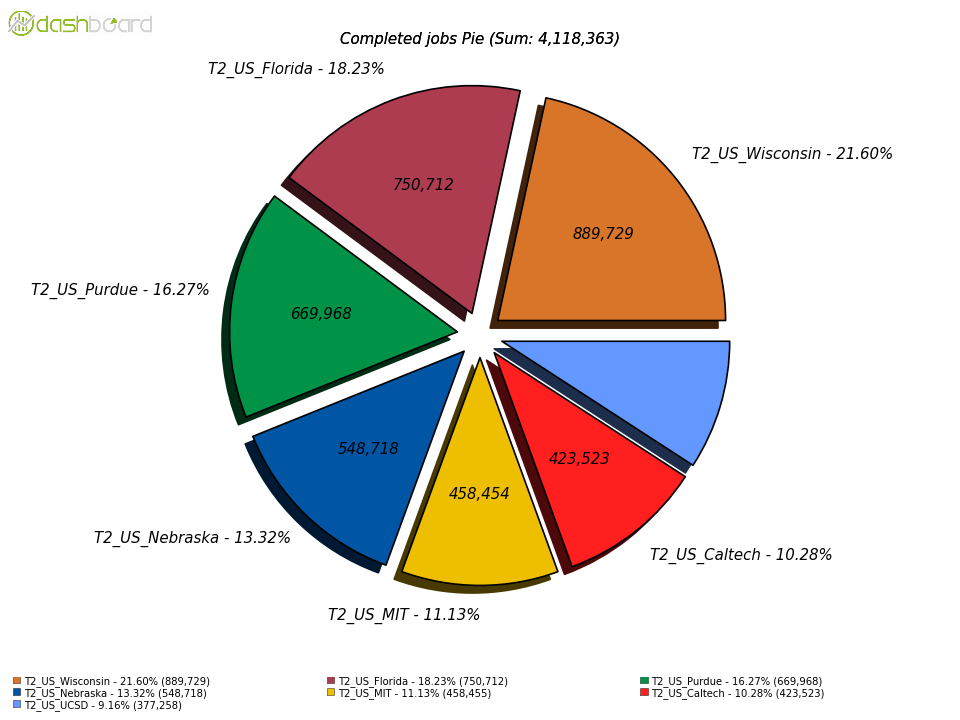
\includegraphics[height=3in]{productionJobsAtUST2sInOneMonth.png}
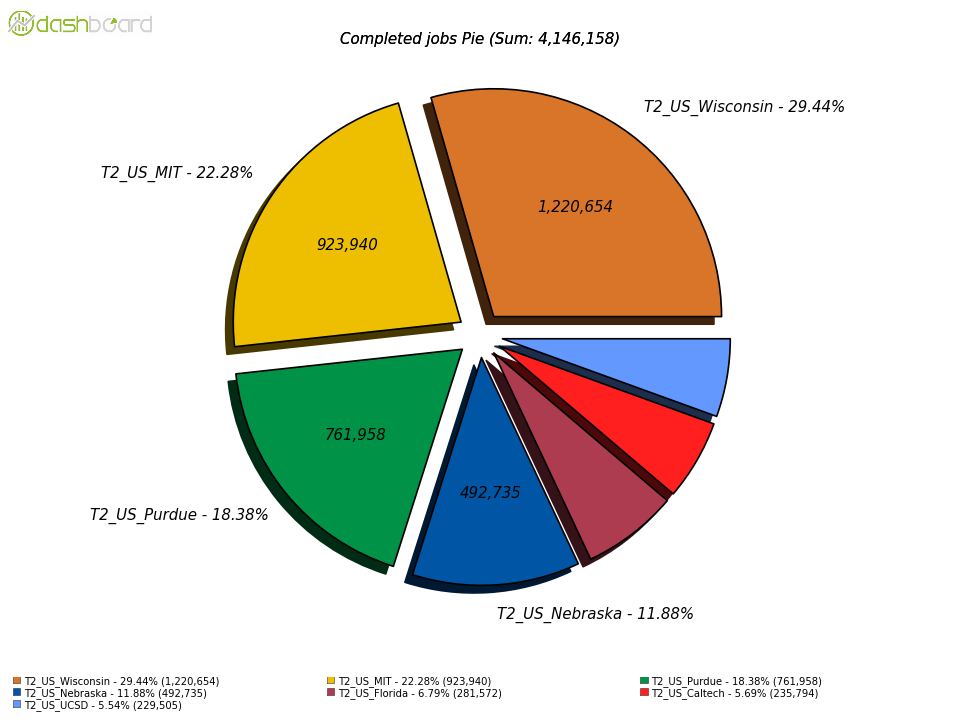
\includegraphics[height=3in]{analysisJobsAtUST2sInOneMonth.png}
\label{computingJobsAtUST2sInOneMonth}
\end{center}
\caption{Counts of completed production (top) and analysis (bottom) 
jobs at the US Tier-2s in the past month (November 2015).}
\end{figure}

\begin{figure}
\begin{center}
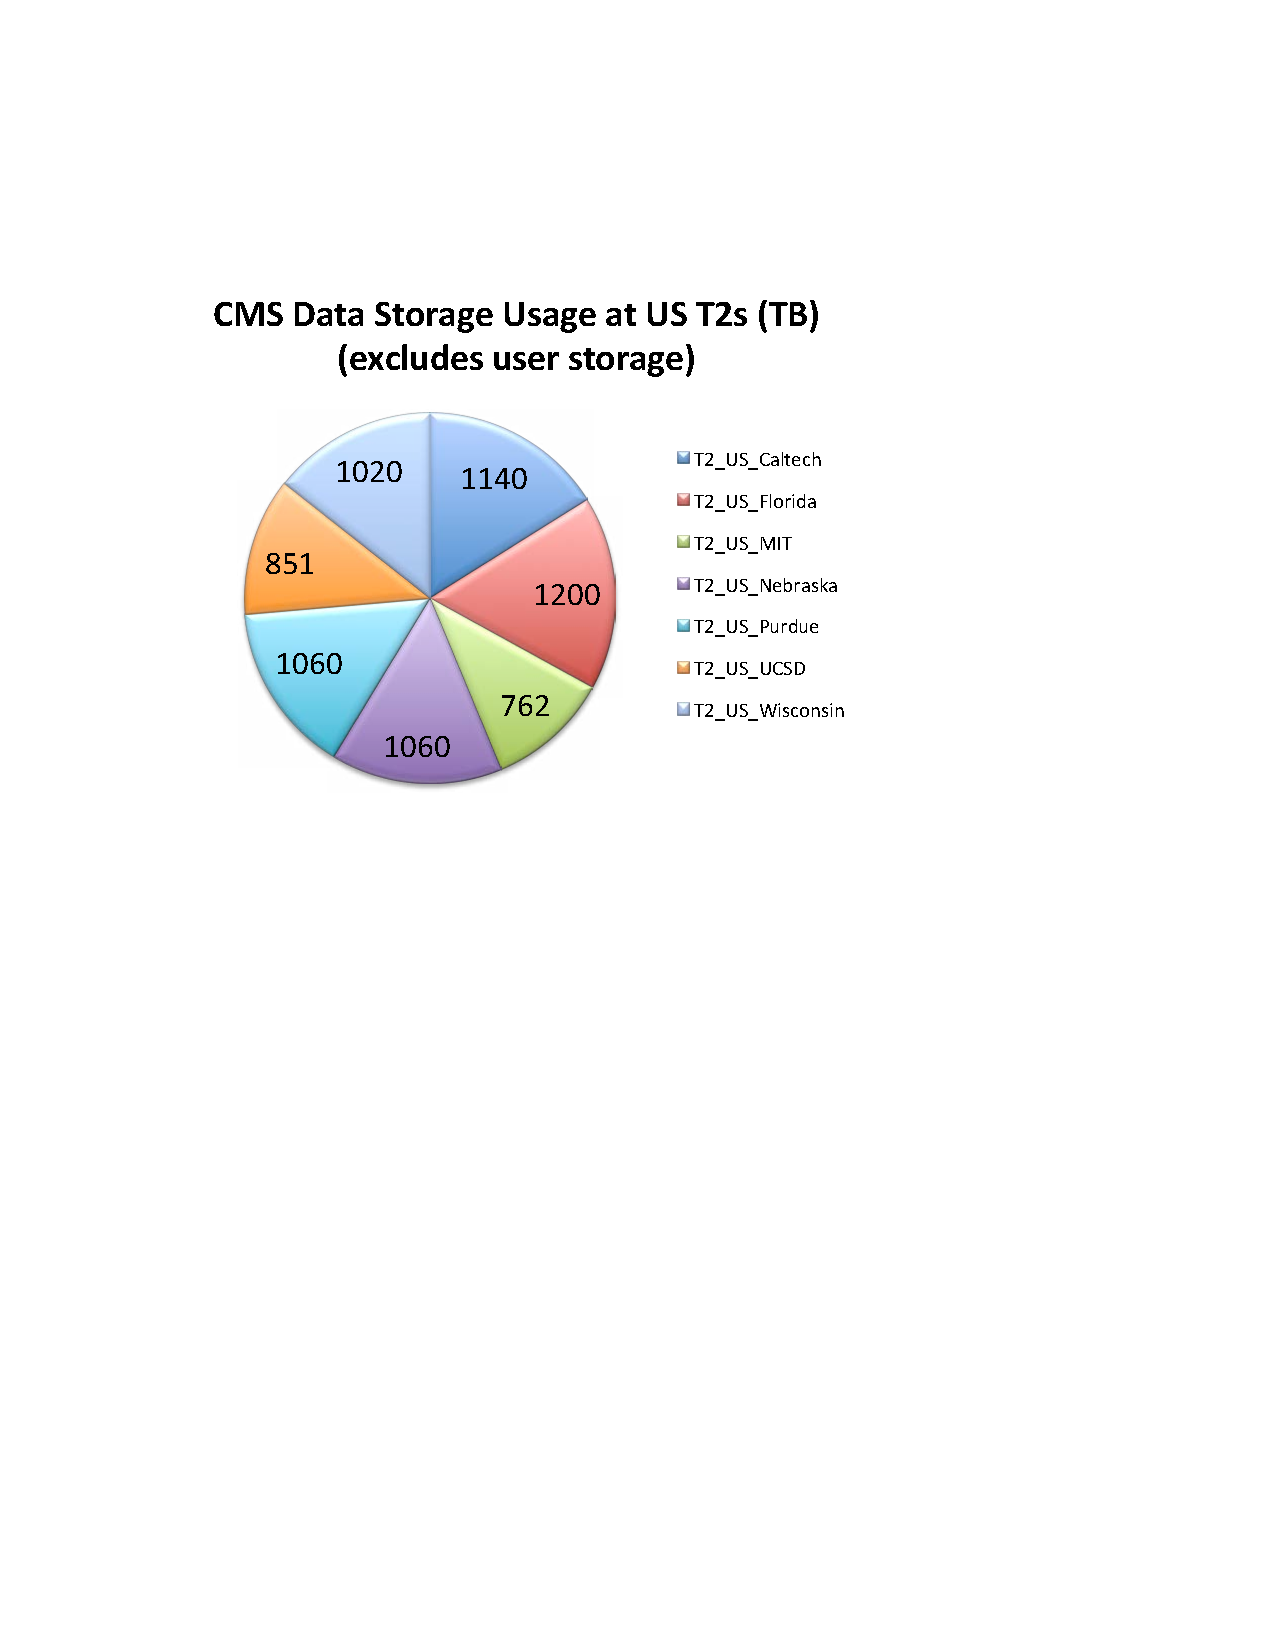
\includegraphics[height=3in]{storageUtilizationAtUST2s-Chart.pdf}
\label{storageUtilizationAtUST2s-Chart}
\end{center}
\caption{Current usage of storage resources for centrally managed
data at the US Tier-2s in the past month (November 2015) in TBs. 
Physicist data storage at each site at the level of about 500 TB
is additional. {\bf fkw: What does this add to the previous table? How does this help the proposal get funded?}}
\end{figure}

\subsubsection{Future Plans}

\noindent{\bf Computing Resources}

To define plans for the future, we start with an extrapolation of needs from the present.

%Unlike for Run-1, the Run-2/3 Tier-2 compute resource provisioning
%details are not concretely specified to allow local optimization based
%on cloud and opportunistic resource availability. However, the
%non-owned storage resource use is not yet well defined. Therefore, it
%is visualized that much of the storage, which is pared down to the
%minimum with improvements made in LS1, is owned and operated at the
%Tier-1s and Tier-2s.

For the sake of simplicity, CPU requirements are estimated in units of number of batch slots
needed based on the following assumptions:

%by scaling current usage up by a factor of 30 accounting for
%increase in expected integrated luminosity.  The increase in
%complexity of analysis is assumed to be compensated by the improved
%framework job efficiency and advances in computing power of individual
%machines.  Use of CMS data federation across the wide-area network at
%owned resource sites and the clouds in general, opens up the
%possibility of provisioning needed compute resources in a flexible way
%depending on cost/benefit.  However, it is visualized that a fraction
%of resources are housed at existing T2s.

\begin{itemize}
\item Currently 30,000 jobs, averaged over the past month, run at the seven 
US T2s equally split between production and analysis and 10,000 production
jobs at FNAL T1.
\item Bulk of the 15,000 analysis jobs running at Tier-2s recently, are 
identified as 13-TeV MC jobs.  The MC for 2015 was generated with the
anticipation that we collect 10 fb$^{-1}$ this year.  While we unfortunately
collected only 2 fb$^{-1}$, we nevertheless consider 10 fb$^{-1}$ the appropriate
integrated luminosity baseline for the needs scaling into the future. 
\item Therefore, scaling by luminosity, 300 fb$^{-1}$ vs 10 fb$^{-1}$ collected 
to date, we should expect to support about 900,000 jobs at T2s at steady state 
and 300,000 jobs at T1.
\item Proposed job slot availability: 300,000 for production at T1 and 100,000 through each of the seven US T2s.
\end{itemize}

\noindent{\bf Storage Resources}

During LS1, CMS introduced a refined analysis format called "MiniAOD".
This format is 1/10th the size of the AOD, and typically requires somewhere between 1/2 to 1/5th the CPU power to
analyze. These reductions are accomplished by storing only more refined information, requiring remaking of the MiniAOD
in response to improved calibrations, or significant improvements of physics objects. During Fall of 2015 CMS went through two iterations
of MiniAOD, with at least one more to follow before Moriond 2016 conference results.
MiniAOD is expected to satisfy the needs of at least 90 \% of all physics analyses. I.e. it is envisioned that a few analyses will
require more detailed information not present in the MiniAOD, and will thus need to access the AOD or maybe even the RAW format.

The operational model today is that Analysis groups process these "primary data" to produce custom 
Ntuples for their analyses at a event processing rate of 1-10Hz or so. The custom Ntuples are then typically 
analyzed at x100 larger event rates. The transformation from primary data useful to the entire collaboration to custom data useful
only to a handful analyses is thus dramatically accelerating science and reducing computing costs with the drawback that non-negligible
amounts of disk space at Tier-2s need to be provisioned to host that custom data. US-CMS organizes this by assigning a fixed set of 
University groups to each Tier-2 as their host Tier-2 for these custom data samples.

The estimated miniAOD size for 300-fb$^{-1}$ of integrated luminosity is:
(50kB)(1kHz) $\times$ (10$^7$s/year) $\times$ (6y) =$3 \times 10^9$
MB=3PB.  Typically to analyze this data requires an associated MC sample which is three times the
size of the detector data, leading to a $\sim$ 12PB disk storage requirement for the CMS data
federation for hosting one replica of one version of all MiniAOD datasets. 
Since the MiniAOD is highly processed it is expected that improvements to the reconstruction,
calibration and other changes will necessitate remaking of MiniAODs.
%Unfortunately, support of multiple versions of MiniAOD for several
%versions, say three, are needed in order to accommodate the analyst
%needs.  
As not all analysts can migrate from one version to another
immediately.  We estimate that two to three MiniAOD versions are
needed at any time, with the older data deprecated dynamically as they
become stale and unused.  This results in an expected disk space requirement of
20-30 PB for MiniAOD for 300-fb$^{-1}$ of integrated luminosity.

In addition to the MiniAOD, we expect to require disk space to accommodate 
$\sim$ 10\% of the data in AOD format on disk to allow the $\le$ 10\% of analyses that require it.
For an AOD event size of $\sim$ 500 kB this amounts to $\sim$ 10PB of storage 
for 300-fb$^{-1}$ of integrated luminosity, or 50 PB total for MiniAOD and AOD combined, allowing some modest
level of replication across sites within the US.
 
For the custom data we project a need of 30PB across the US-CMS Tier-2s based on our Run1 experience.
This data is not replicated, nor is it assumed to be backed up to tape. Implicit in this operational model is the assumption that the data
can be reproduced easily enough if lost due to disk failures at a Tier-2.

In addition to data analysis activities of the Run2 and Run3 data, we also must budget for disk space for the CMS upgrade activities.
We expect event sizes to be larger, and a more heavy use of AOD as upgrade activities will be focused around custom simulations
and detailed reconstruction development. We budget 20 PB for the purpose of the present needs assessment.

Finally, there is a need for some RAW data on disk, plus staging space to in front of the Tier-1 tape archive, as well as at the Tier-2s for 
staging data as it is being reconstructed or simulations as they are being produced. Based on our present experience, we assume
10PB to be sufficient to accommodate this.

Adding it all up, we arrive at a total disk space need of 110PB at US-CMS facilities for 300 fb$^{-1}$ of integrated luminosity, 
and we are proposing to locate 12PB of this at each of the seven US Tier-2s.
There is no tape storage at Tier-2 centers today, and we expect to keep it that way. Tape needs are thus out of scope for the present proposal
and thus not discussed here.

\noindent{\bf Network Resources}

The network bandwidth requirement will also scale with increased data
size and wide-area distributed computing.  Typically sites are
connected through 100 Gbps network presently, and we expect
multi-100 Gbps connections in the coming years. Up to now, networking at Tier-2 centers has always been funded
via sources outside the US-CMS software and computing project. We expect this to stay that way, and are thus not budgeting
any costs for networking as part of this proposal.

\noindent{\bf Non-traditional resources beyond Tier-1 and Tier-2}

In the last few years, NSF-ACI made some very substantial investment
into networking infrastructure across more than 100 campuses
nationwide. Among them are 25 of the 40 collaborating universities in
US-CMS. We propose to build on this NSF investment by working with all
of them, as well as any of the remaining 15 universities interested,
to fully integrate their campus IT operated hardware infrastructures
and ScienceDMZs into the US-CMS Tier-2 infrastructure. This will be
done following the model of the NSF funded ``Pacific Research
Platform'' (PRP) using Open Science Grid (OSG) tools and processes.
The PRP deploys single nodes into the ScienceDMZs of 20 institutions
across the West Coast, including the US-CMS institutions UC Davis, UC
Santa Barbara, UC Riverside, Caltech, and UC San Diego. These pieces
of hardware are collaboratively maintained between the campus IT
organizations and the PRP and SDSC teams at UCSD such that local IT is
responsible for hardware and user account maintenance, and UCSD is
responsible for all OS and software service maintenance.  The
functionality implemented includes interactive data analysis, batch
submission, CVMFS software cache, XRootd data cache, and XRootd server
to export local data. The hardware is effectively a Tier-3 in a box
without any of the human maintenance needs from the local CMS
community. The deployment model includes careful custom integration
into any existing University clusters accessible to the local
group. This is made manageable with minimal effort beyond the initial
deployment by management of OS, US-CMS and OSG services, and local
configurations via a central Puppet infrastructure at UCSD.

The local CMS community is thus empowered to transparently use any and
all local resources the University allows them to share in combination
with the entire Tier-1 and Tier-2 system. Official CMS data is cached
locally as needed. Private data by the local community is served out
to the Tier-1 and Tier-2 system via XRootd servers. Each Tier-2 will
also have an XRootd cache in order to transparently cache the private
data of any of the local communities to avoid IO latencies due to WAN
reads given the finite speed of light.  The HTCondor batch systems
implemented on these pieces of hardware are all connected to the
global CMS HTCondor pool via glideinWMS. Similarily any University
clusters are integrated requiring nothing more than ssh access to a
US-CMS account on the local University cluster. Sharing policies are
controlled locally following local rules at each University. We expect
that some Universities will enable access to all of US-CMS to share
their spare capacity, while others will be more restrictive. All of
this is presently already deployed and operated by PRP and SDSC for
the US-ATLAS group at UC Irvine, and is being deployed at the CMS
institutions listed above. Operations for the UC groups is funded via
a mix of NSF and state funds. We are proposing to scale out deployment
and operations of this model across the US to as many US-CMS
institutions as possible, focusing on the 25 institutions that have
received ScienceDMZ funding from NSF-ACI since 2012. The hardware
costs as well as the human effort to deploy and operate this system
will be borne out of the Tier-2 portion of this proposal. At a cost of
$\sim$\$10,000 per Tier-3 in a box, this is a modest fraction of the
total Tier-2 hardware budget across the seven Tier-2s and the 5 years
of this proposal.

We fully understand that the above model will not be appropriate for
all 40 collaborating institutions within US-CMS. We thus augment it
with an additional hosted service build on the OSG-connect model
pioneered by the University of Chicago OSG/ATLAS group.  This service
will provide identical functionality to the Tier-3 in a box for
institutions that are either lacking appropriate network connectivity
or a local IT organization that would be capable and/or willing to
collaborate on the hardware and user account maintenance.  There will
be only a single instance of this "CMS-Connect" infrastructure for all
these remaining groups. Groups within US-CMS are thus generally better
off with a Tier-3 in a box, especially when they have sizable private
data collections and large groups of students and post-docs. 

Finally, we will fully integrate cloud services access into this
infrastructure in such way that local University groups can use local
funds to purchase cloud resources to augment their personal access to
computing resources, and thus accelerate their science. We expect to
be collaborating on this functionality with the HEPCloud project at
FNAL as well as the Open Science Grid.

In addition to all of the above functionality geared towards data
analysis, we propose to also integrate Supercomputing resources at DOE
and NSF funded national facilities mostly for the purpose of
simulation and reconstruction, i.e. the production of the official CMS
datasets.  Again, we expect to collaborate heavily with HEPCloud and
OSG on the detailed access mechanisms and policies.  At this point,
December 2015, HEPCloud is focused on AWS, while OSG is working with
Comet (NSF) and Cori (DOE) to understand the technical, operational,
and security processes for use of these supercomputers via OSG
interfaces.

\noindent{\bf Facilities Support Personnel}

Two persons at each facility are necessary to provide full coverage.
However, recent experience indicates that about 30-50\% of those
person's effort can be freed up for other work. Most of the effective
people involved in CMS computing are former HEP physicists, who have
now become experts in computing. They are able to provide wide-ranging
expertise in physics software development.  The additional services we
expect Tier-2 personnel to provide are in the areas:
\begin{itemize}
\item Support for non-Tier-2 university portals to CMS cloud
\begin{itemize}
\item We expect each Tier-2 to support about 7 universities in their neighborhood.
\end{itemize}
\item Computing services for CMS upgrades and research to address future needs
\begin{itemize}
\item Development of simulation program for upgrade detectors
\item Production of simulation data for upgrade detectors
\item Participation in computing research
\item Participation in DIANA/HEP and other community wide computing projects for future.
\end{itemize}
\end{itemize} 

\subsection{Operations (WBS 3)}

In addition to operating the Tier-2 facilities, additional S\&C 
operations functions are met by the personnel supported by this
project.  

\subsubsection{Current Status}

Currently these additional operations include support for Frontier
database at Johns Hopkins.  Frontier provides run conditions and other
configuration information for reconstruction and analysis jobs running
on our distributed infrastructure.  It also includes support for
software distribution at Florida.  The grid-wide job submission
infrastructure operations at UCSD and AAA operations at Nebraska. The
biggest item is the T0 operations at MIT and CERN.  Cost of living
adjustment for those working on T0 operations at CERN is also
included.  Support for simulations production at Wisconsin is also
currently included here.

\subsubsection{Future Plans}

The Tier-0 operations remain essentially the same, requiring continued
support of personnel both at MIT and at CERN.  As we scale higher in
both job slots and their distribution over the CMS cloud, and highly
distributed storage access on the WAN using AAA technologies
underlying the CMS data federation, we anticipate that these
operations support remain.  Additional operations support for smooth
operation of US university portals (Tier-3-in-a-box) and efficient
harnessing of opportunistic resources is also anticipated.

\subsection{Computing Infrastructure and Services (WBS 4)}

The US CMS S\&C institutions continue to develop new solutions for CMS
computing problems that result in more efficient use of both storage
resources, using dynamic data management and seamless wide-area
network access to our storage (AAA and XROOTD), and compute resources,
using improved workflows.  For instance, data management and workflow 
management development is done at Cornell, xrootd development at
UCSD, and dynamic data placement development at MIT.  Additional 
support was provided by NSF through AAA project to Nebraska, UCSD
and Wisconsin.

\subsubsection{Current Status}

\noindent{\bf Dynamic Data Placement and Management}

Underpinning the computing infrastructure in Run-1 was data
distribution mechanism implemented using PhEDEx software. The workflow
involved operators moving large chunks of data on command down the
hierarchical grid so that after initial calibration and reconstruction
at Tier-0, the raw data were moved to be archived at Tier-1 and
reprocessed as necessary. The (re)reconstructed data from Tier-1s were
further processed to obtain lower volume Analysis Objects Data (AOD)
versions whose copies were transferred to Tier-2s and placed on disk
storage for random access for chaotic analysis workflows.  Similarly
the Monte Carlo (MC) simulation data was produced at Tier-2s,
aggregated, reconstructed and archived at Tier-1s. The MC AODs were
then placed on command by the operators at various Tier-2s. The net
result was multiple copies of data placed statically at various
facilities around the globe. It was observed that much of the disk
volume was occupied by often rarely used data.

Dynamic data placement and management (DDM) software was developed and
commissioned during the LS1 to address these shortcomings. DDM is now
deployed at all tiers to automatically prune the unused but archived
data using well defined policies.  For example, the archived full
event, i.e., raw plus reconstructed quantities (FEVT) is pruned from
disk to keep sufficient space for the Tier-0 and Tier-1 reconstruction
workflows to execute smoothly. Most importantly we are able to keep at
least one copy of all AOD on disk somewhere in the CMS data
federation, and duplicate multiple times as needed for popular data.

\noindent{\bf CMS Data Federation (AAA)}

CMS Data Federation is built to provide seamless international-scale data
access  under the auspices of Any Data, Anytime, Anywhere
(AAA) project. AAA removes the requirement of co-location of storage and
processing resources.  The infrastructure is transparent, in that
users have the same experience whether the data they analyze is
halfway around the world or in the room next door.  It is reliable, in
that end users never see a failure of data access when they run their
application.  It enables greater access to the data, in that users no
longer have the burden of purchasing and operating complex disk
systems. In fact, any data can be accessed anytime from anywhere with
an internet connection. The key to success of AAA is the improved
wide-area network access due to enhancements made to our dedicated LHC
network.

AAA is made possible by XRootd software, which allows the creation of
data federations. A data federation serves a global namespace via a
tree of XRootd servers. The leaves of this tree are referred to as
data sources, as they serve data from the local storage systems.
Each storage system is independent of the others, allowing for a broad
range of implementations and groups to participate in the federation
as long as they expose an agreed-upon namespace through the XRootd
software. The non-leaf nodes have no storage, but may redirect client
applications to a subscribed data source that has the requested file.
Each host is subscribed to at most one redirector, called a manager;
loops are disallowed. If the requested file is not present on a server
subscribed to the redirector, then the client will be redirected to
the current host's manager.  The manager continues the process until
either a source is found or the client is at the root of the tree. An
application may thus be redirected to any host in the federation,
irrespective of the branch point it initially accesses.

CMS Data Federation is now fully deployed across all tiers of its
computing infrastructure. Easy access to this data federation across
the wide-area network is democratizing the computing abilities of
University groups across the world. Local campus grids controlled by
non-CMS entities are easily integrated in the CMS computing
environment. Temporary access to dedicated large resources can be
purchased on commercial grids or obtained from national or campus
research facilities.

\noindent{\bf Development of MiniAOD}

Physics analysis often involves a much smaller portion of
reconstructed data than is available. While the raw data acquired from
CMS is about 1 MB per event, the reconstructed objects more than
double that size typically. The AOD defined for Run-1 was successful
but was designed in a rather lax way resulting in a 400 kB size per
event, which when scaled to 300 fb$^{-1}$ results in unaffordable
data volume. Further, rate of event processing matters in time to
production of physics results, so size of event being small is also
beneficial for computational loads. 

The US CMS personnel supported by NSF played key role in development
of the MiniAOD.  Careful pruning of unused collections of objects, packing them
in appropriately sized containers resulted in redefined miniAOD which
is less than 50 kB per event. The miniAOD is now visualized as the main data format that will
be used by bulk of CMS analysts, while niche usecases involving the
original AOD format will be supported as needed. In rare cases FEVT
access may also be needed.  As the miniAOD improves we anticipate AOD
replica counts will become small. 

\noindent{\bf Improvements to CMS Workflows}

The main objectives of the workflows management middleware is to
process data as quickly as possible, maintain uniform load across all
resource sites and enable fast recovery in case of a site service
interruption, e.g., by relocating jobs on an alternate site, while
keep track of the integrity of the combined dataset.  Recent
developments in workflow management enable CMS to utilize impermanent
opportunistic resources for data production. These workflow changes
are enabling CMS to take better advantage of owned and opportunistic
resources.  For instance the ability to use the high-level trigger
farm for MC production and reconstruction during the down periods of
time. Recent tests indicate ability to switch to offline processing
workflows within several minutes. Improved data transfer technology
and remote Xrootd access to CMS data federation are enabling
technologies.

\noindent{\bf Opportunistic Resources}

CMS is in exploratory phase for smoothly integrating opportunistic
resources for production and routine use. National research computing
sites such as NERSC and SDSC have large resources, but often requiring
additional work in adaptation of our software suite to smoothly
operate there. Some access restrictions are worked around with user
level code, e.g., CVMFS through Parrot and Docker/Shifter containers
on Cray supercomputers. Commercial clouds such as AWS have also been
used, but have cost-implications placing constraints on workflows. For
example, the stage-out of data over the network is expensive. We have
adapted by chaining various stages of workflow so that the smallest
useable unit, say miniAOD is the only output that is staged out to the
CMS data federation. Non-owned campus clusters are accessible both
through their OSG connection if existing generically, or by placing
suitable head-nodes at the participating university CMS group
facilities. This latter use is of particularly important for analysis
groups at access their home resources seamlessly processing data from
the central CMS data federation using centrally supported code and
conditions repositories using technologies such as CVMFS and caching
SQUIDs. The CMS HLT cloud using virtual machines technology is able to
quickly bring in very large resource during data taking down periods
for offline workflow processing. Some of the innovations made there
are useable elsewhere.

Final stages of physics analysis often involve workflows that are not
centrally managed CMSSW framework jobs. Technologies such as CMS
Connect are able to use campus grid and department level computer
clusters to bring additional opportunistic uses for these cases.

\subsubsection{Future Plans}

Blah Blah Blah indicating that continued in R\&D of {Computing Infrastructure and Services (WBS 4)}
is necessary.

\subsection{Software and Support (WBS 5)}

Multicore computing systems have become ubiquitous in the past
decade. However, efficient use of available resources, especially
memory volume and access, required adaptation of our software to
suitable multithreaded frameworks. Keeping up with technology
evolution in the market requires continues investigation and CMS
framework and utilities software development.  Cornell, Princeton and
UCSD groups are engaged with central CMS in this essential software
development and support.

\subsubsection{Current Status}

A systematic effort to make the core CMSSW thread-safe and has
successfully deployed it in the past year.  The event display
for CMS has been reworked to work on a variety of platforms
conveniently.

\subsubsection{Future Plans}

{FIXME: We need to list what is required to be done by the people
  supported by this WBS.}

\subsection{Technologies and Upgrade R\&D (WBS 6)}

The main thrust of the R\&D effort of the project is to control the
rate of growth of computing used.  High-Luminosity is the least
pleasant way to go exploring. Unlike high(er) energy, one has to cope
with increased event size (due to pile-up), pile-up complexity
increases due to many overlapping events, data set size increases due
to long running period required, impacting CPU, storage and network
resources.  For example, an increase in number of PU events from 10-25
was measured to result in increase of a x3 of event reconstruction
time. Such size increases (or larger) are unaffordable and must be
prevented.

\subsubsection{Current Status}

Tuning of multi-threaded software to increase the resource
usage efficiency is one of our recent accomplishments.  
{FIXME: Add more from David and Liz, when ready}

\subsubsection{Future Plans}

There are a few possible ways to deal with this set of challenges. 
\begin{itemize}
\item reduce size/event e.g. miniAOD and beyond. Study operational and Physics implications.
\item speed up reconstruction time, using vectorization and parallelization enabled by the new computing architectures. 
\item explore the limitations of AAA. Start on US-side.  
\end{itemize}

Invsetigation of new computing architectures, re-engineering of
reconstruction for use on HPC machines, impact of reduced data formats
like miniAOD and beyond are all on the list of items to be tackled.
At Princeton efforts in reconstruction on new architectures is
beginning Cornell has begun efforts on new architectures and data
mining.  Nebraska and Wisconsin have long standing collaborations with
distributed high-throughput computing experts from their CS
departments.  Caltech software engineers are also formulating R\&D
plans for long term, in collaboration with the CERN based multicore
projects.

Long term R\&D in exploring options of using GPUs for extensive
parallel processing is under investigation.  While some of the long
term R\&D is supported externally, we anticipate that rapid deployment
of newly available products, which will certainly be necessary will
require additional investment within the US CMS S\&C project.


\subsection{Coordination with CMS (WBS 7)}

US CMS S\&C personnel are well inetgrated in the CMS-wide coordination
efforts and hold management positions.  

\subsubsection{Current Status}

Current support under this category includes S\&C coordination at
Princeton, reconstruction coordination at Wisconsin and UCSD, and user
support at UCSD.  

\subsubsection{Future Plans}

It is anticipated that approximately a third of the management positions
in CMS are held by US personnel, of which NSF computing supported 
personnel needs will have to be covered by this project.  The need
is likely to remain approximately constant.

\end{document}

\end
